\def\tg{\mathrm{tg}}
\def\cotg{\mathrm{cotg}}
\def\arctg{\mathrm{arctg}}
\def\arccotg{\mathrm{arccotg}}

\section{Základy diferenciálního počtu}

\begin{pozadavky}
\begin{pitemize}
	\item Reálné funkce jedné reálné proměnné
	\item Spojitost, limita funkce v bodě (vlastní i nevlastní)
	\item Některé konkrétní funkce (polynomy, racionální lomené funkce, goniometrické a cyklometrické funkce, logaritmy a exponenciální funkce)
	\item Derivace: definice a základní pravidla, věty o střední hodnotě, derivace vyšších řádů
	\item Některé aplikace (průběhy funkcí, Newtonova metoda hledání nulového bodu, Taylorův polynom se zbytkem)
\end{pitemize}
\end{pozadavky}

\subsection{Reálné funkce jedné reálné proměnné}
\begin{definiceN}{Reálná funkce}
Reálná funkce jedné proměnné je zobrazení $f: M \rightarrow \mathbb{R}$, kde $M \subseteq \mathbb{R}$. \\
$f$ je na $M$:
\begin{pitemize}
	\item \emph{rostoucí}: $\forall x, y: x < y \Rightarrow f(x) < f(y)$
	\item \emph{klesající}: $\forall x, y: x < y \Rightarrow f(x) > f(y)$
	\item \emph{neklesající}: $\forall x, y: x < y \Rightarrow f(x) \le f(y)$
	\item \emph{nerostoucí}: $\forall x, y: x < y \Rightarrow f(x) \ge f(y)$

	\item \emph{sudá}: $x \in M \Rightarrow -x \in M \wedge f(x)=f(-x), \forall x \in M$
	\item \emph{lichá}: $x \in M \Rightarrow -x \in M \wedge f(x)=-f(-x), \forall x \in M$
	\item \emph{periodická} s periodou $p\in\mathbb{R}$: $x \in M \Rightarrow x \pm p \in M \wedge f(x)=f(x+p)=f(x-p), \forall x \in M$
\end{pitemize}
\end{definiceN}

\begin{definiceN}{Okolí bodu}
$P(a, \delta) = (a-\delta, a) \cup (a, a+\delta)$ (prstencové okolí)

\noindent
$P^{+}(a, \delta)=(a, a+\delta)$ (pravé prstencové okolí)

\noindent
$P^{-}(a, \delta)=(a-\delta, a)$ (levé prstencové okolí)

\noindent
$B(a, \delta)=(a-\delta, a+\delta) = P(a, \delta)+\{a\}$ ($\delta$-okolí)

\noindent
Podobně se definuje i levé a pravé $\delta$-okolí bodu $a$.
\end{definiceN}

\subsection{Spojitost, limita funkce v bodě (vlastní i nevlastní)}

\begin{definiceN}{Limita}
Řekneme, že $f$ má v bodě $a \in \mathbb{R}^{*}$ limitu $A \in \mathbb{R^{*}}$, jestliže
$$\forall \varepsilon>0\ \exists \delta>0: \forall x \in P(a, \delta) \Rightarrow f(x) \in B(A, \varepsilon)$$
a značíme $\lim_{x \rightarrow a} f(x) = A$

\medskip
Platí-li tato vlastnost jen pro pravá okolí bodů $a$ a $A$, mluvíme o \emph{jednostranné limitě zprava} a podobně zleva.
\end{definiceN}

\begin{definiceN}{Spojitost v bodě}
Řekneme, že $f$ je spojitá v bodě $a \in \mathbb{R}$, jestliže $\lim_{x \rightarrow a} f(x) = f(a)$
\end{definiceN}

\begin{vetaN}{Heineho věta}
Nechť  $f: M \rightarrow \mathbb{R}, M \subseteq \mathbb{R}$. Nechť $f$ je definováno na nějakém prstencovém okolí bodu $a \in \mathbb{R}^{*}$. Potom následující dvě tvrzení jsou ekvivalentní:
\begin{penumerate}
	\item $lim_{x \rightarrow a} f(x) = A \in \mathbb{R}^{*}$
	\item Pro každou posloupnost $\{x_n\}_{n=1}^{\infty}$ splňující $x_n \in D(f)\ \forall n \in \mathbb{N}$ a  $\lim x_n = a, x_n \neq a\ \forall n$ platí $\lim_{n \rightarrow \infty} f(x_n)=A$
\end{penumerate}
Heineho věta umožňuje tvrzení, vyslovená o limitách posloupností, převádět na limity funkcí v bodě.
\end{vetaN}

\begin{vetaN}{Věta o jednoznačnosti limity funkce}
Funkce $f$ má v každém bodě nejvýše jednu limitu.
\end{vetaN}

\begin{vetaN}{O lokální omezenosti funkce s vlastní limitou}
Nechť funkce $f$ má v bodě $a \in \mathbb{R}^{*}$ vlastní limitu. Potom existuje $\delta > 0$ takové, že $f$ je na $P(a, \delta)$ omezená.
\end{vetaN}

\begin{vetaN}{Aritmetika limit pro funkce}
Nechť $\lim_{x \rightarrow a} f(x)=A$, $\lim_{x \rightarrow a} g(x)=B$, $a \in R^{*}$. Potom
\begin{penumerate}
	\item $\lim (f(x)+g(x)) = A+B$, je-li výraz na pravé straně definován.
	\item $\lim (f(x)g(x)) = A\cdot B$, je-li výraz na pravé straně definován.
	\item $\lim \frac{f(x)}{g(x)} = \frac{A}{B}$, je-li výraz na pravé straně definován.
\end{penumerate}
\end{vetaN}

\begin{vetaN}{Limita a uspořádání - policajti pro funkce}
\begin{penumerate}
	\item Nechť $\lim_{x \rightarrow a} f(x) > \lim_{x \rightarrow a} g(x)$, $a \in R^{*}$.\\Potom $\exists P(a, \delta): f(x)>g(x) \ \forall x \in P(a, \delta)$
	\item Nechť $f(x) \le g(x), \forall x \in P(a, \delta), \delta > 0$ a existují $\lim_{x \rightarrow a} f(x)$, $\lim_{x \rightarrow a} g(x)$.\\Potom $\lim_{x\to a} f(x) \le \lim_{x\to a} g(x)$.
	\item Nechť $f(x) \le h(x) \le g(x), \forall x \in P(a, \delta), \delta > 0$ a $\lim_{x \rightarrow a} f(x) = \lim_{x \rightarrow a} g(x)$.\\Potom existuje $\lim h(x)$ a $\lim_{x \rightarrow a} h(x) = \lim_{x \rightarrow a} f(x) = \lim_{x \rightarrow a} g(x)$.
\end{penumerate}
Pozor na ostrost nerovností, v tomto případě je velmi důležitá.
\end{vetaN}

\begin{definiceN}{Jednostranná spojitost funkce v bodě}
\begin{pitemize}
	\item $\textit{funkce f je spojitá v a} \Leftrightarrow \lim_{x \rightarrow a} f(x)=f(a) \Leftrightarrow \forall \varepsilon>0~\exists \delta >0: f(B(a, \delta)) \subseteq B(f(a), \varepsilon)$
	\item $\textit{funkce f je spojitá v a zprava} \Leftrightarrow \lim_{x \rightarrow a^{+}} f(x)=f(a) \Leftrightarrow \forall \varepsilon>0~\exists \delta >0: f(B^{+}(a, \delta)) \subseteq B(f(a), \varepsilon)$
	\item $\textit{funkce f je spojitá v a zleva} \Leftrightarrow \lim_{x \rightarrow a^{-}} f(x)=f(a) \Leftrightarrow \forall \varepsilon>0~\exists \delta >0: f(B^{-}(a, \delta)) \subseteq B(f(a), \varepsilon)$
\end{pitemize}
\end{definiceN}

\begin{vetaN}{O limitě složené funkce}
Nechť $\lim_{x \rightarrow a} g(x) = A$, $\lim_{y \rightarrow A} f(y) = B$, $a, A, B \in \mathbb{R}^{*}$. Nechť navíc platí jeden z předpokladů:\\
(P1) $f$ je spojitá v $A$\hfill \textit{(vnější funkce je spojitá)}\\
(P2) $\exists \delta > 0: g(x) \neq A$ pro $\forall x \in P(a, \delta)$\hfill \textit{(vnitřní je \uv{lokálně prostá})}\\
Potom $\lim_{x \rightarrow a} (f \circ g)(x) = B$.
\end{vetaN}

\begin{definiceN}{Interval}
Nechť $a, b \in \mathbb{R}^{*}, a < b$. Pak \emph{otevřeným intervalem} $(a, b)$ nazveme $\{x | a<x<b\}$, \emph{(uzavřeným) intervalem} $\left<a, b\right>$ (pro $a, b \in \mathbb{R}$) nazveme $I=\{x | a \le x \le b\}$. Uzavřený interval se někdy značí i $[a,b]$.
\end{definiceN}

\begin{vetaN}{Věta o limitě monotónní funkce}
Nechť je funkce $f$ monotónní na $(a, b)$, $a, b \in \mathbb{R}^{*}, a < b$. Potom $\exists \lim_{x \rightarrow a^{+}} f(x)$, $\exists \lim_{x \rightarrow b^{-}} f(x)$.
\end{vetaN}

\begin{definiceN}{Spojitost na intervalu}
Je-li $\left<a, b\right>$ interval, pak $a$ nazýváme počátečním bodem, $b$ koncovým bodem a $x \in (a, b)$ vnitřními body.

Řekneme, že $f$ \emph{je spojitá na intervalu $I$}, jestliže je spojitá zprava ve všech bodech kromě koncového a spojitá zleva ve všech bodech kromě počátečního.
\end{definiceN}

\begin{vetaN}{O spojitém obrazu intervalu}
Nechť funkce $f: I \rightarrow \mathbb{R}$ je spojitá na intervalu $I$. Potom $f(I)$ je také interval.
\end{vetaN}

\begin{vetaN}{Darbouxova o nabývaní mezihodnot}
Nechť funkce $f$ je spojitá na $\left<a, b\right>$ a $f(a)<f(b)$, potom $\forall y \in (f(a), f(b))$ existuje $x \in (a, b)$ takové, že $f(x)=y$.
\end{vetaN}

\begin{definice}
$f: M \rightarrow \mathbb{R}, M \subseteq \mathbb{R}$. $f$ nabývá v bodě $a \in M$:
\begin{pitemize}
	\item \emph{maxima} na M $\Leftrightarrow \forall x \in M: f(x) \le f(a)$
	\item \emph{minima} na M $\Leftrightarrow \forall x \in M: f(x) \ge f(a)$
	\item \emph{ostrého maxima} na M $\Leftrightarrow \forall x \in M\setminus \{a\}: f(x) < f(a)$
	\item \emph{ostrého minima} na M $\Leftrightarrow \forall x \in M\setminus \{a\}: f(x) > f(a)$
	\item \emph{lokálního} maxima (minima, ostrého...)$\Leftrightarrow \exists \delta > 0: f$ nabývá na $M \bigcap B(a, \delta)$ maxima (minima, ...)
\end{pitemize}
\end{definice}

\begin{vetaN}{Vztah spojitosti a extrémů}
Nechť $f$ je spojitá na $\left<a, b\right>$. Potom $f$ nabývá na $\left<a, b\right>$ svého maxima i minima.
\end{vetaN}

\begin{vetaN}{Vztah spojitosti a omezenosti}
Spojitá funkce na uzavřeném intervalu $\left<a, b\right>$ je omezená.
\end{vetaN}

\begin{definiceN}{prostá funkce, inverzní funkce}
Funkce $f$ je \emph{prostá}, jestliže $\forall x, y \in D(f): x \neq y \Rightarrow f(x) \neq f(y)$.

Nechť $f$ je prostá na $M$, tedy $f: M \rightarrow f(M)$. Pak \emph{inverzní funkce} $f^{-1}$ k funkci $f$ je definovaná na $f(M)$ předpisem: $y \in f(M)$, pak $f^{-1}(y)=x \Leftrightarrow y=f(x)$.
\end{definiceN}

\begin{vetaN}{O inverzní funkci}
Nechť $I$ je interval a funkce $f$ je definovaná, spojitá a rostoucí (klesající) na $I$. Potom inverzní funkce $f^{-1}$ je definována, spojitá a rostoucí (klesající) na $f(I)$.
\end{vetaN}

\subsection{Některé konkrétní funkce (polynomy, racionální lomené funkce, goniometrické a cyklometrické funkce, logaritmy a exponenciální funkce)}

\begin{vetaN}{Exponenciální funkce}
Existuje právě jedna reálná funkce \textbf{exp}, splňující:
\begin{pitemize}
	\item $\exp(x+z)=\exp(x) \exp(z), \forall x,z \in \mathbb{R}$
	\item $\exp(x) \ge 1+x, \forall x \in \mathbb{R}$
\end{pitemize}
\end{vetaN}

\begin{poznamkaN}{Některé vlastnosti $\exp$}
Platí:
\begin{pitemize}
    \item $\exp 0=1$
    \item $\exp (-x) = \frac{1}{\exp x}$
    \item $\exp (x) \neq 0\ \forall x\in \mathbb{R}$
    \item $\lim_{x\to\infty}\exp x=\infty$, $\lim_{x\to-\infty}\exp x=0$
    \item $\exp$ je rostoucí na $\mathbb{R}$
    \item $\lim_{x\to 0}\frac{\exp x - 1}{x}=1$
\end{pitemize}
\end{poznamkaN}

\begin{vetaN}{Vlastnosti $\log$}
Funkce $\log$, definovaná předpisem $\log=\exp^{-1}$ má následující vlastnosti:
\begin{pitemize}
	\item $D(\log)=(0, \infty)$, $\log ((0, \infty)) \rightarrow \mathbb{R}$
	\item $\log(x\cdot y) = \log x + \log y, \forall x, y \in (0, \infty)$, $\log(x^n)=n\log x$
	\item log je spojitá, rostoucí na $(0, \infty)$, $\log 1=0$, $\log e = 1$
	\item $lim_{x \rightarrow 0_{+}} \log x = - \infty$, $lim_{x \rightarrow \infty} \log x = \infty$
	\item $lim_{x \rightarrow 1} \frac{\log x}{x-1} = 1$, $lim_{x \rightarrow 0} \frac{\log x+1}{x} = 1$
\end{pitemize}
\end{vetaN}

\begin{definiceN}{obecná mocnina}
Obecná mocnina $a^b=\exp(b \log a)$ pro $a>0, b \in \mathbb{R}$. Speciálně pro $a=e: e^x=\exp x$
\end{definiceN}

\begin{veta}
Existuje právě jedna reálná funkce $s$ a právě jedna reálná funkce $c$ taková, že:

\begin{pitemize}
	\item $s(x+y) = s(x)c(y) + c(x)s(y)$
	\item $c(x+y) = c(x)c(y) - s(x)s(y)$
	\item $s$ je lichá, $c$ sudá
	\item $s>0~\textit{na}~(0,1), s(1)=0$
\end{pitemize}
\end{veta}

\begin{definice}
\noindent Podle $s$ a $c$ definujeme \emph{Goniometrické funkce}:\\
$\sin(x)=s(\frac{x}{\pi})$, $\cos(x)=c(\frac{x}{\pi})$, $\tg(x)=\frac{\sin(x)}{\cos(x)}$, $\cotg(x)=\frac{\cos(x)}{\sin(x)}$

\noindent \emph{Cyklometrické funkce}:
\begin{pitemize}
	\item $\arcsin x = y \Leftrightarrow y \in <-\frac{\pi}{2}, \frac{\pi}{2}> \wedge \sin y=x$
	\item $\arccos x = y \Leftrightarrow y \in <0, \pi> \wedge \cos y=x$
	\item $\arctg~x = y \Leftrightarrow y \in (-\frac{\pi}{2}, \frac{\pi}{2}) \wedge \tg~y=x$
	\item $\arccotg~x = y \Leftrightarrow y \in (0, \pi) \wedge \cotg~y=x$
\end{pitemize}

\noindent a platí
$$\lim_{x \rightarrow 0} \frac{\arcsin x}{x} = 1$$
$$\lim_{x \rightarrow 0} \frac{\arccos x}{\sqrt{1-x}} = \lim_{x \rightarrow 0} \frac{\arctg x}{x} = 1$$
\end{definice}

\subsection{Derivace: definice a základní pravidla, věty o střední hodnotě, derivace vyšších řádů}
\begin{definice}
Nechť $f$ je reálná funkce jedné proměnné, $a \in \mathbb{R}$. Derivací funkce $f$ v bodě $a$ nazveme
$$f'(a) = \lim_{h \rightarrow 0} \frac{f(a+h)-f(a)}{h} \textrm{, pokud existuje}$$

\noindent Derivací zprava a zleva rozumíme:
$$f'_{+}(a) = \lim_{h \rightarrow 0_+} \frac{f(a+h)-f(a)}{h}, \, f'_{-}(a) = \lim_{h \rightarrow 0_-} \frac{f(a+h)-f(a)}{h}$$
\end{definice}

\begin{vetaN}{Vztah derivace a spojitosti}
Má-li $f$ v $a$ vlastní derivaci, potom je $f$ v $a$ spojitá.
\end{vetaN}

\begin{vetaN}{Aritmetika derivací}
Nechť existují $f'(a)$, $g'(a)$:
\begin{penumerate}
	\item $(f+g)'(a)=f'(a)+g'(a)$, je-li pravá strana definována
	\item je-li $g$ nebo $f$ spojitá v $a$, pak $(fg)'(a)=f'(a)g(a)+f(a)g'(a)$
	\item je-li $g$ spojitá v $a$, $g(a) \neq 0$, pak $(\frac{f}{g})'(a)=\frac{f'(a)g(a)-f(a)g'(a)}{g^2(a)}$
\end{penumerate}
\end{vetaN}

\begin{vetaN}{O derivaci složené funkce}
Nechť funkce $f$ má derivaci v $y_0$, $g$ má derivaci v $x_0$, $g$ je spojitá v $x_0$ a $y_0=g(x_0)$. Potom $(f \circ g)'(x_0)=f'(y_0)\cdot g'(x_0)=f'(g(x_0))\cdot g'(x_0)$.
\end{vetaN}

\begin{vetaN}{O derivaci inverzní funkce}
Nechť funkce $f$ je na intervalu $(a,b)$ spojitá a ryze monotonní a má v bodě $x_0 \in (a,b)$ derivaci $f'(x_0)$ vlastní a různou od nuly. Potom má funkce $f^{-1}$ derivaci v bodě $y_0=f(x_0)$ a platí rovnost
$$(f^{-1})'(y_0) = \frac{1}{f'(f^{-1}(y_0))}.$$
\begin{poznamka}
Pokud v situaci popsané v právě uvedené větě je $f'(x_0)$ nevlastní, je $(f^{-1})'(y_0)=0$. Je-li $f'(x_0)=0$, je $(f^{-1})'(y_0)=+\infty$ (je-li $f$ rostoucí), resp. $=-\infty$ (je-li $f$ klesající).
\end{poznamka}
\end{vetaN}

\begin{vetaN}{Nutná podmínka lokálního extrému}
Nechť $M \subseteq \mathbb{R}$, $f: M \rightarrow \mathbb{R}$. Nechť $f$ má v $a \in M$ lokální extrém. Pak buď neexistuje $f'(a)$, nebo $f'(a)=0$.
\end{vetaN}

\begin{vetaN}{Rolleova věta}
Nechť $f$ je spojitá na $\left<a, b\right>$ a nechť existuje $f'(x)\ \forall x \in (a,b)$. Nechť $f(a)=f(b)$. Potom existuje $\xi \in (a,b): f'(\xi)=0$.
\end{vetaN}

\begin{vetaN}{Lagrangeova o střední hodnotě}
Nechť $f$ je spojitá na $\left<a, b\right>$ a nechť existuje $f'(x)\ \forall x \in (a,b)$. Potom existuje $$\xi \in (a,b): f'(\xi)=\frac{f(b)-f(a)}{b-a}$$
\end{vetaN}

\begin{vetaN}{Cauchyova o střední hodnotě}
Nechť $f$ a $g$ jsou spojité na $\left<a, b\right>$, nechť existuje $f'(x)\ \forall x \in (a,b)$ a nechť existuje $g'(x)$ vlastní a nenulové. Potom existuje $$\xi \in (a,b): \frac{f(b)-f(a)}{g(b)-g(a)}=\frac{f'(\xi)}{g'(\xi)}$$

\begin{dukaz}
$g(a) \neq g(b)$, neboť jinak by podle Rolleovy věty existovalo $\xi \in (a,b): g'(\xi)=0$. Definujeme $H(x)=(f(x)-f(a))(g(b)-g(a))-(g(x)-g(a))(f(b)-f(a))$. Potom $H(a)=H(b)=0$, $H$ je spojitá na $\left<a, b\right> \Rightarrow \exists H' na (a,b)$. Tedy podle Rolleovy věty $\exists \xi: 0 = H'(\xi)=f'(\xi)(g(b)-g(a))-g'(\xi)(f(b)-f(a))$. Tedy $\frac{f(b)-f(a)}{g(b)-g(a)}=\frac{f'(\xi)}{g'(\xi)}$, neboť $g'(\xi) \neq 0$ a $g(b)-g(a)\neq 0$ 
\begin{flushright}$\square$\end{flushright}
\end{dukaz}
\end{vetaN}

\begin{vetaN}{L'Hospitalovo pravidlo}
\csprimeson
Nechť $a \in \mathbb{R}^{*}$ a funkce $f$, $g$ jsou definovány na nějakém $P(a, \delta)$, $f, g$ mají v $P(a,\delta)$ vlastní derivaci, $\forall x \in P(a,\delta): g'(x)\not=0$ a existuje $\lim_{x \rightarrow a} \frac{f'(x)}{g'(x)}$. Nechť platí i jedna z následujících podmínek:
\begin{penumerate}
	\item $\lim_{x \rightarrow a} f(x)=\lim_{x \rightarrow a} g(x)=0$
	\item $\lim_{x \rightarrow a+} |g(x)|=+\infty$
\end{penumerate}
Potom existuje i $\lim_{x \rightarrow a} \frac{f(x)}{g(x)}$ a platí $\lim_{x \rightarrow a} \frac{f(x)}{g(x)}=\lim_{x \rightarrow a} \frac{f'(x)}{g'(x)}$.
\end{vetaN}

\begin{vetaN}{O limitě derivací}
Nechť funkce $f$ je spojitá zprava v $a \in \mathbb{R}$ a nechť existuje $\lim_{x \rightarrow a_+} f'(x)=A \in \mathbb{R}^*$. Potom $f'_+(a)=A$.
\end{vetaN}

\begin{vetaN}{Vztah derivace a monotonie}
Nechť $I$ je nezdegenerovaný interval (tj. nejde o jediný bod) a $Int(I)=\{\textit{vnitřní body I}\}$. Nechť $f$ je spojitá na $I$ a existuje $f'$ vlastní na $Int(I)$.:
\begin{penumerate}
	\item je-li $f' > 0$ na $Int(I)$, pak f je rostoucí na I
	\item je-li $f' \ge 0$ na $Int(I)$, pak f je neklesající na I
	\item je-li $f' < 0$ na $Int(I)$, pak f je klesající na I
	\item je-li $f' \le 0$ na $Int(I)$, pak f je nerostoucí na I
\end{penumerate}
\end{vetaN}

\begin{definiceN}{Tečna, inflexe}
Nechť funkce $f$ má v $a \in \mathbb{R}$ vlastní derivaci. Označíme $T_a=\{[x,y]\in \mathbb{R}^2, y=f(a)+f'(a)(x-a)\}$. Řekneme, že $[x, f(x)] \in \mathbb{R}^2$ leží nad (pod) tečnou $T_a$, jestliže $f(x)>f(a)+f'(a)(x-a)$ ($f(x)<f(a)+f'(a)(x-a)$).

Nechť $f$ má v $a \in \mathbb{R}$ vlastní derivaci. Řekneme, že $f$ má v $a$ \emph{inflexi}, jestliže $\exists \delta > 0$: buď $\forall x \in (a-\delta, a): [x, f(x)]$ leží nad $T_a$ $\wedge$ $\forall x \in (a, a+\delta): [x, f(x)]$ leží pod $T_a$, nebo opačně.
\end{definiceN}

\begin{vetaN}{Nutná podmínka existence inflexe}
Jestliže $f''(a) \neq 0$, pak $f$ nemá v $a$ inflexi.
\end{vetaN}

\begin{vetaN}{Postačující podmínka existence inflexe}
Nechť $f$ má spojitou první derivaci na $(a,b)$. Nechť $z \in (a,b)$. Nechť $\forall x \in (a,z): f''(x)>0$ a $\forall x \in (z, b): f''(x)<0$ (nebo naopak). Pak $z$ je bod inflexe $f$.
\end{vetaN}

\begin{definice} % definice se x_1,x_2,x_3 je podle me srozumitelnejsi, ale jak myslis ... -- Tuetschek
Řekneme, že funkce $f$ je na intervalu $I$:
\begin{pitemize}
	\item \emph{konvexní}, jestliže pro každé $x_1, x_2 \in I$ a každé $\lambda \in \left<0, 1\right>$ platí\\$f(\lambda x_1 + (1-\lambda)x_2) \le \lambda \cdot f(x_1)+(1-\lambda)\cdot f(x_2)$.
	\item \emph{konkávní}, jestliže pro každé $x_1, x_2 \in I$ a každé $\lambda \in \left<0, 1\right>$ platí\\$f(\lambda x_1 + (1-\lambda)x_2) \ge \lambda \cdot f(x_1)+(1-\lambda)\cdot f(x_2)$.
	\item \emph{ryze konvexní}, jestliže pro každé $x_1, x_2 \in I, x_1 \neq x_2$ a každé $\lambda \in (0, 1)$ platí\\$f(\lambda x_1 + (1-\lambda)x_2) < \lambda \cdot f(x_1)+(1-\lambda)\cot f(x_2)$.
	\item \emph{ryze konkávní}, jestliže pro každé $x_1, x_2 \in I, x_1 \neq x_2$ a každé $\lambda \in (0, 1)$ platí\\$f(\lambda x_1 + (1-\lambda)x_2) > \lambda \cdot f(x_1)+(1-\lambda)\cdot f(x_2)$.
\end{pitemize}
\end{definice}

\begin{veta}
Nechť funkce $f$ je konvexní na $I$ a $a \in Int(I)$. Potom $\exists f'_+(a) \in \mathbb{R}$ a $\exists f'_-(a) \in \mathbb{R}$. Tj. konvexnost implikuje existenci vlastních jednostranných derivací, neznamená to ale, že existuje derivace.
\end{veta}

\begin{vetaN}{Vztah konvexity a spojitosti}
Nechť $f$ je konvexní na otevřeném intervalu $(a, b)$. Pak $f$ je na $(a, b)$ spojitá.
\end{vetaN}

\begin{veta}
Nechť $f$ má spojitou první derivaci na $I=(a, b)$. Potom:
\begin{pitemize}
	\item $f''(x)>0\ \forall x \in (a, b)$, pak f je ryze konvexní na $(a, b)$
	\item $f''(x) \ge 0\ \forall x \in (a, b)$, pak f je konvexní na $(a, b)$
	\item $f''(x)<0\ \forall x \in (a, b)$, pak f je ryze konkávní na $(a, b)$
	\item $f''(x) \le 0\ \forall x \in (a, b)$, pak f je konkávní na $(a, b)$
\end{pitemize}
\end{veta}

\begin{definiceN}{Asymptota}
Funkce $f$ má \textit{asymptotu} $ax+b$ v $+\infty$ $(-\infty)$, jestliže $f$ je definována na nějakém okolí $+\infty (- \infty)$ a platí
$$\lim_{\substack{x \rightarrow \infty \\ (x \rightarrow -\infty)}} (f(x)-ax-b)=0$$
\end{definiceN}

\begin{vetaN}{Výpočet asymptoty}
Funkce $f$ má v $\infty$ asymptotu $ax+b$, právě když $$\lim_{x \rightarrow \infty}\frac{f(x)}{x}=a \in \mathbb{R},\,\lim_{x \rightarrow \infty}(f(x)-ax)=b \in \mathbb{R}$$
Analogicky pro $- \infty$.
\end{vetaN}

\subsection{Některé aplikace (průběhy funkcí, Newtonova metoda hledání nulového bodu, Taylorův polynom se zbytkem)}

\subsubsection*{Vyšetření průběhu funkce:}
\begin{penumerate}
	\item Určíme definiční obor a obor spojitosti funkce.
	\item Zjistíme symetrie: lichost, sudost, periodicita.
	\item Dopočítáme limity v \uv{krajních bodech definičního oboru}.
	\item Spočítáme první derivaci (tam, kde existuje, případně jednostranné derivace), určíme intervaly monotonie a nalezneme lokální a globální extrémy. Určíme obor hodnot.
	\item Spočteme druhou derivaci a určíme intervaly, kde funkce f je konvexní nebo konkávní. Určíme inflexní body.
	\item Vypočteme asymptoty funkce.
	\item Načrtneme graf funkce.
\end{penumerate}

\subsubsection*{Taylorův polynom se zbytkem}

\begin{definice}
Nechť $f$ je reálná funkce, $a \in \mathbb{R}$, $n \in \mathbb{N}$ a $f$ má derivace do řádu $n$. Pak funkci
$$T^{f,a}_n(x)=f(a) + f'(a)(x-a) + \dots + \frac{f^{(n)}(a)}{n!}(x-a)^n$$
nazýváme \emph{Taylorovým polynomem funkce $f$ řádu $n$ v bodě $a$}.
\end{definice}

\begin{veta}
Nechť $f$ je reálná funkce, $a \in \mathbb{R}$, nechť existuje vlastní $f^{(n)}(a)$. Nechť $P$ je polynom stupně $\le n$. Pak $$\lim_{x \rightarrow a} \frac{f(x)-P(x)}{(x-a)^n}=0 \Leftrightarrow P=T^{f,a}_{n}$$
\end{veta}

\begin{vetaN}{Obecný tvar zbytku}
Nechť $f$ má vlastní (n+1)-ní derivaci v intervalu $\left<a,x\right>, x>a$. Nechť $\varphi$ je spojitá funkce na $\left<a,x\right>$, která má na $(a,x)$ vlastní nenulové derivace. Pak:
$$\exists \xi \in (a, x): R^{f,a}_{n}(x)=f(x)-T^{f,a}_n(x)=\frac{1}{n!}.\frac{\varphi(x)-\varphi(a)}{\varphi'(\xi)}.f^{(n+1)}(\xi).(x-\xi)^n$$

\begin{dukaz}
Věta je důsledkem Cauchyho věty o střední hodnotě, aplikované na funkci $F(t):=f(x)-T^{f,t}_n(x)$, definované pro $t\in[a,x]$. (Ošklivou a pracnou) derivací této funkce vyjde, že $F'(t) = -\frac{f^{(n+1)}(t)}{n!}(x-t)^n\ \forall t\in(a,x)$ a teď použijeme onu Cauchyho větu a dostaneme 
$$\frac{-\frac{f^{(n+1)}(\xi)}{n!}(x-\xi)^n}{\varphi'(\xi)} = \frac{F'(\xi)}{\varphi'(\xi)} = \frac{F(x)-F(a)}{\varphi(x)-\varphi(a)} = \frac{0-R_n^{f,a}(x)}{\varphi(x)-\varphi(a)}$$
což už dává kýžený tvar zbytku.
\begin{flushright}$\square$\end{flushright}
\end{dukaz}
\end{vetaN}

\begin{dusledek}
\emph{Lagrangeův tvar zbytku}:
Je-li $\varphi(t)=(x-t)^{n+1}$, dostaneme
$$R^{f,a}_{n}(x)=\frac{1}{(n+1)!} f^{(n+1)}(\xi) (x-a)^{n+1}$$
\emph{Cauchyho tvar zbytku}:
Je-li $\varphi(t)=t$, dostaneme
$$R^{f,a}_{n}(x)=\frac{1}{n!} f^{(n+1)}(\xi) (x-\xi)^{n} (x-a)$$
\end {dusledek}

\subsubsection*{Newtonova metoda hledání nulového bodu}
Zdroje: \\
\texttt{http://www.kvd.zcu.cz/cz/materialy/numet/\_numet.html\#\_Toc501178905},\\ 
\texttt{http://www.mojeskola.cz/Vyuka/Php/Learning/Derivace/matika\_krokem5.php} :-)

\medskip
Newtonova metoda je numerická...

Jde o nalezení nulového bodu nějaké funkce, tedy bodu, kde $f(x) = 0$ pro nějakou reálnou funkci $f$ na intervalu $\left<A,B\right>$.

Jako první aproximaci ($x_1$) kořene rovnice v intervalu $\left<A,B\right>$ použijeme střed tohoto intervalu. V něm sestrojíme tečnu a její průsečík s osou $x$ je novou aproximací ($x_2$) kořene. V tomto bodě sestrojíme opět tečnu atd.

Další, přesnější, novou aproximaci kořene tedy hledáme jako průsečík tečny ve staré aproximaci s osou $x$.

Máme-li řešit rovnici $f(x) = 0$, pak rovnice tečny ve starém průsečíku ($x_n$) bude $y - f(x_n) = f'(x_n)(x - x_n)$
Průsečík s osou $x$ získáme vyjádřením $x$ z rovnice: $0 - f(x_n) = f'(x_n)(x - x_n)$ Tedy: $x = x_n - \frac{f(x_n)}{f'(x_n)}$
Tento průsečík bude novou aproximací ($x_{n+1}$) kořene.

Výsledný vztah pro výpočet nové aproximace tedy zní: 
$$x_{n+1} = x_n - \frac{f(x_n)}{f'(x_n)}$$

Lze očekávat při každé iteraci dojde ke zdvojnásobení počtu platných číslic. Pro odhad chyby lze použít vzorec $\textit{chyba} \le \frac{|f(x_i)|}{m}$, kde $m$ je minimum hodnoty první derivace v intervalu od počáteční aproximace ke kořeni. Nevýhodou této metody je ovšem to, že nemusí konvergovat vždy. Také kriterium použitelnosti může značně omezit oblast jejího používání:
\begin{pitemize}
	\item funkce musí být v okolí kořene spojitá
	\item funkce nesmí mít v okolí kořene nulovou derivaci a musí být splněna podmínka $\left|\frac{f(x)f''(x)}{[f'(x)]^2}\right| \le m < 1$
\end{pitemize}

Řešení je pro konvexní i konkávní funkce stejné, pouze je zapotřebí jinak volit výchozí bod. U konvexních funkcí je zapotřebí zvolit výchozí bod nad očekávaným kořen a přibližovat se k němu shora. U konkávních funkcí je třeba zvolit výchozí pod kořenem a ke kořenu se přibližovat zdola. Princip Newtonovy metody pro konvexní funkce je znázorněn na následujícím obrázku:

\begin{center} 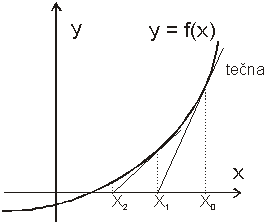
\includegraphics[width=4cm]{matematika/obrazky/newton.png} \end{center}
